\section{Primo punto: Phishing e AUR}
\label{sec:primo-punto}
La compromissione dell'account è iniziata da una mail inviata da un account chiamato support@npmjs.help, dominio registrato in Olanda appena tre giorni prima dell'attacco.
\begin{figure}[H]
    \centering
    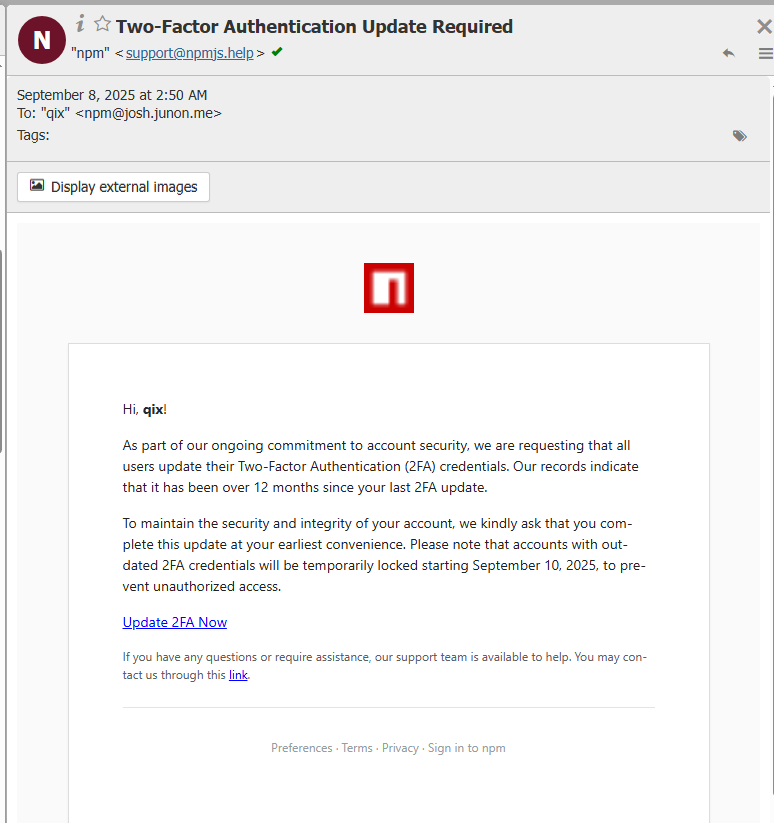
\includegraphics[width=0.85\textwidth, height=0.4\textheight]{mail_phishing.png}
    \caption{Mail di phishing ricevuta dall'utente.}
    \label{fig:phishing}
\end{figure}
Dal testo si puo notare subito un dettaglio sospetto: entro 2 giorni l'account verrà sospeso se non si effettua il login, un chiaro tentativo di creare urgenza e pressione psicologica sull'utente.

Qualche ora dopo, più precisamente alle 13:16 UTC, i sistemi di Aikido, un'azienda specializzata in cybersecurity, hanno scoperto che l'account di josh stava pubblicando pacchetti con vulnerabilità note, e che quindi era stato compromesso. 
Lo stesso utente ha dichiarato poche ore dopo di aver perso l'accesso al proprio account e di essere stato ingannato siccome la mail era molto credibile e lui aveva passato una settimana stressante, il che lo ha reso disattento e vulnerabile.
Tutti i pacchetti compromessi contenevano codice javascript che intercettava e dirottava sia il traffico web che quello API cercando indirizzi di wallet di criptovalute. 
Quando veniva trovato un indirizzo di un wallet, il codice lo sostituiva con un indirizzo controllato dall'attaccante per poter reindirizzare i fondi verso il proprio wallet. 
Per rendere piu difficile la comprensione del codice malevolo, l'attaccante ha utilizzato tecniche di offuscamento del codice come l'uso di variabili con codici come per esempio la variabile 0x112fa8.

\begin{figure}[H]
    \centering
    \includegraphics[width=0.85\textwidth, height=0.4\textheight]{codice_malevolo.png}
    \caption{estratto del codice malevolo presente nei pacchetti compromessi}
    \label{fig:phishing}
\end{figure}

% Inserire spiegazioni, esempi ed eventuali riferimenti con \cite{chiave}.
